\section{Durchführung}
\label{sec:Durchfuehrung}

\subsection{Einseitige Einspannung}
\label{sec:einseiteEinspannung}
Mit Hilfe des in Abbildung \ref{fig:aufbau} gezeigten Versuchsaufbaus lässt sich der Elastizitätsmodul bestimmen.
Dabei werden zwei Stäbe mit kreisförmigen und quadratischen Querschnitt in die Apparatur einseitig bei A eingespannt 
und mit einem am Stabende befestigten Gewicht gebogen.
Die Auslenkung des Stabs an einem Punkt wird mit einer Messuhr bestimmt. Die Messuhr lässt sich entlang der Apparatur
verschieben und die Entfernung vom Einspannpunkt ist oben auf der Apparatur anhand einer Längenskala ab zu lesen.

\begin{figure}
    \centering
    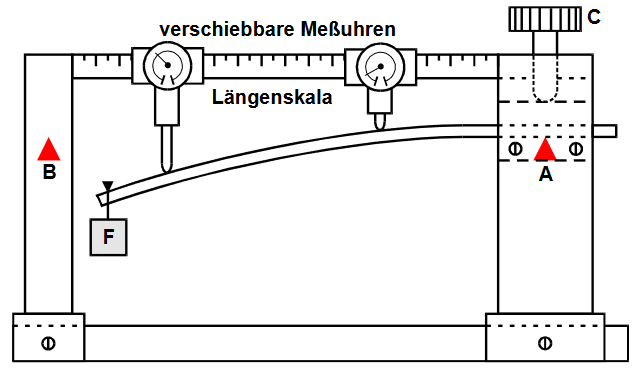
\includegraphics[width=0.7\textwidth]{aufbau.png}
    \caption{Schematische Aufbau der Apparatur \cite{anleitung}.}
    \label{fig:aufbau}
\end{figure}

Da nicht davon ausgegangen werden kann, dass die Stäbe komplett gerade sind, wird eine Nullmessung durchgeführt, um
die tatsächliche Biegung zu bestimmen.

\subsection{Beidseitige Auflage}
\label{sec:beidseitigeEinspannung}
Nun werden die Stäbe nacheinander bei A und bei B aufgelegt und das Gewicht in der Mitte des Stabs befestigt. Es wird dabei
wieder eine Nullmessung durchgeführt. Bei der Messung ist zu beachten, dass beide Messuhren verwendet werden, da die Befestigung
der Masse die Bewegung der Messuhr über die Mitte nicht zulässt.